\documentclass[letterpaper, 10pt, english, conference]{IEEEtran}

\overrideIEEEmargins

\usepackage{amsfonts}
\usepackage{amsmath,amssymb}
\usepackage[tight]{subfigure}
\usepackage{cite}
\usepackage[vlined,linesnumbered,ruled]{algorithm2e}
\usepackage{color}

\ifx\pdfoutput\undefined
\usepackage{graphicx} % not running pdftex
\else
\ifx\pdfoutput\relax
\usepackage{graphicx} % not running pdftex
\else
\ifnum\pdfoutput>0
\usepackage[pdftex]{graphicx} % running pdftex with pdf output
\else
\usepackage{graphicx} % running pdftex with dvi output
\fi
\fi
\fi

\usepackage{verbatim}
\newtheorem{theorem}{Theorem}
\newtheorem{problem}{Problem}


%\makeatletter
%%%%%%%%%%%%%%%%%%%%%%%%%%%%%% User specified LaTeX commands.
%\usepackage[T1]{fontenc}
%\usepackage{pslatex}

%\makeatother

%\usepackage{babel}
\begin{document}

\global\long\def\at#1{}

\newcommand{\rrtstar}{RRT$^*$ }

%\title{\LARGE \bf Optimal Sampling-Based Planning with Automatically
%  Derived Extension Procedures for Systems with General Costs and
%  Dynamics}
%\title{\LARGE \bf LQR-RRT* for Systems with General Costs and Dynamics}
\title{\LARGE \bf Optimal Sampling-Based Planning for General Kinodynamic Systems}

\author{
\authorblockN{Gustavo Goretkin, Alejandro Perez, Robert Platt Jr., and George Konidaris; TLPK?}
\authorblockA{Computer Science and Artificial Intelligence Laboratory,
Massachusetts Institute of Technology\\
\{goretkin, aperez, rplatt, gdk\}@csail.mit.edu}
}

\maketitle

\begin{abstract}
We introduce a method for automatically deriving the cost metric and
steering method--- critical components of the RRT$^*$
algorithm---for general kinodynamic systems with differentiable dynamics and twice
differentiable cost functions. We first introduce a version of the
RRT$^*$ algorithm that uses an LQR-based extension to plan for
problems with affine dynamics and second order costs, and prove that
it almost surely converges to the optimal plan.  We then show how to
automatically derive a cost metric and extension method for problems
with nonlinear dynamics and non-quadratic costs by locally
approximating both functions. 
%This allows us to automatically derive
%an extension method for general domains, provided their dynamics are
%locally differentiable and their cost function locally twice
%differentiable. 
This removes the need for domain-specific extension
methods, which are a major obstacle to the general applicability of
RRT$^*$.  
%We demonstrate our method's application in a few standard
%benchmark domains.
\end{abstract}

\section{Introduction}

The RRT$^*$ algorithm \cite{karaman.frazzoli.ijrr11} offers a
practical and effective method for probabilistically complete optimal
motion planning.  Like all members of the RRT family of planning
algorithms \cite{lavalle.kuffner.ijrr01} it incrementally builds a
tree by using a cost measure to determine the ``closest'' vertices in the
tree to a random sample, and a steering method to find an
extension
trajectory from a given node in the tree to 
the sample. Designing such procedures is
straightforward for kinematic systems, but it is much more
challenging for kinodynamic systems because it is non-trivial to calculate 
good local 
%locally optimal 
kinodynamic trajectories, even in free space. Hence, 
designing the
distance measure and steering method often represents the major obstacle
to applying RRT$^*$ to kinodynamic systems.

Since control theory offers methods for exactly computing 
optimal policies and the corresponding cost-to-go functions for linear systems
with quadratic costs
(using the linear quadratic regulator, or LQR, family of solution methods),
several researchers have applied LQR-based methods
to estimate distance and to calculate locally optimal
trajectories, as originally suggested by LaValle and Kuffner
\cite{lavalle.kuffner.ijrr01}. 
%
Glassman and Tedrake 
used an affine version of LQR to 
estimate kinodynamic distance
between a random sample and vertices in an RRT~\cite{elena.russ.icra10}.
 Perez et al.~\cite{Perez12} extended
that idea to the RRT$^*$ setting using an
infinite-horizon LQR controller that both estimated 
the cost and calculated trajectories for extending the tree. 
Unfortunately, due to its use of an infinite horizon LQR controller,
this steering method does not always yield
locally optimal trajectories for the finite-time extensions (even for
linear systems). 
Webb and van den Berg~\cite{jur} 
used a finite-horizon optimal controller to calculate the extension
trajectories, obtaining the optimal finite time-horizon by
finding the roots of a high-order polynomial. In conjunction with
RRT$^*$, this steering method was proven to converge to optimal
solutions for linear systems problems with indefinite time
horizons. Unfortunately, this method requires
a very specific type of quadratic cost function.
%is complex to implement because
%of the root-finding requirements and can only be used with a very
%specific type of quadratic cost function. 
Moreover, it is not clear
how it could be extended to non-linear problems,
where the
root-finding method would not apply.

We propose a new method for automatically deriving the cost
metric and steering method for general kinodynamic
systems using affine LQR. We avoid the problem of
determining the optimal time horizon to use for LQR when extending
the tree by 
including time as an additional dimension of the space in which the
tree grows. This approach is sometimes
used to solve problems with dynamic obstacles
environments~\cite{lavalle.book06,stillman?}. In our case, the
purpose is to sample from the space of possible trajectory
durations. Although this can increase the
asymptotic computational complexity of the algorithm, it eliminates
the need to calculate an optimal extension time horizon using
special-purpose tools, while remaining applicable to 
%It is therefore simultaneously
%much simpler to implement and
%enlarges the space of problem specifications that can be
%solved. 
We show that this method trivially satisfies
Karaman and Frazzoli's requirements for probabilitic optimality of the
<<<<<<< Updated upstream
resulting trajectory, when the system has linear dynamics and 
quadratic costs. We also show how to use locally linear dynamic
and locally quadratic cost approximations to apply the method
to general kinodynamic systems. 
We provide simulations illustrating the behavior of the
algorithms for both linear systems with quadratic costs,
and in more general settings.

\section{Background}

\section{Background}
\subsection{Problem Statement}

Given a deterministic system with known process dynamics, the optimal
kinodynamic motion planning problem is to find a trajectory that
begins in a given start state, terminates in a goal region, avoids
obstacles, and satisfies differential dynamics constraints. Let the
state space and control input space of the system be described by
compact sets, $X \subseteq \mathbb{R}^n$ and $U \subseteq
\mathbb{R}^m$, respectively. The system process dynamics are described
by a continuously differentiable function,
\begin{equation}
\dot{x}(t) = f(x(t),u(t)),
\label{eqn:sys_dynamics}
\end{equation}
where $x(t) \in X$ and $u(t) \in U$. Given a time horizon, $T \in
\mathbb{R}_{>0}$, a dynamically feasible trajectory is a continuous
function, $x: [0,T] \to X$, for which there exists a control function,
$u:[0,T] \to U$, that satisifies Equation~\ref{eqn:sys_dynamics}. The
optimal kinodynamic motion planning problem is to find a dynamically
feasible trajectory starts in an initial state, $x_0 \in X$, avoids
obstacles, $X_{obs} \subset X$, and terminates in a goal region,
$x_{goal} \subset X$ while minimizing a cost functional of
Equation~\ref{eqn:cost_fn}.

\begin{problem}
\label{prob:1}
(Optimal kinodynamic motion planning~\cite{Karaman.Frazzoli:CDC10})

Given a state space, $X$, obstacle region, $X_{obs}$, goal region,
$X_{goal}$, control input space, $U$, and function $f$ describing the
system process dynamics, find a control, $u : [0,T] \to U$, for some $T
\in \mathbb{R}_{>0}$ such that the corresponding dynamically feasible
trajectory, $x : [0,T] \to X$, avoids the obstacle region, reaches the
goal region, and minimizes the cost functional
\begin{equation}
J(x,u) = \int_{t=0}^T g(x(t),u(t)).
\label{eqn:cost_fn}
\end{equation}

\end{problem}


\subsection{RRT$^*$}

The Optimal Rapidly-Exploring Random Tree (RRT$^*$) \cite{karaman.frazzoli.ijrr11} is a version of the RRT algorithm~\cite{lavalle.kuffner.ijrr01} that has the \emph{asymptotic optimality} property, i.e., almost-sure convergence to an optimal solution.

The algorithmic primitives are:
\begin{itemize}
\item {\it Random sampling}:
%
The ${\tt Sample}$ procedure provides independent uniformly distributed random samples of states from the configuration space.

\item {\it Nearest nodes}:
%
Given a set $V$ of vertices in the tree and a state $x$, the ${\tt
Nearest}(V, x)$ procedure provides the state in $V$ that is closest to
$x$. 

\item {\it Near nodes}:
%
Given a set $V$ of vertices in the tree and a state $x$, the ${\tt
Near}(V, x)$ procedure provides a set of states in $V$ that are close to
$x$. Here, closeness is measured with respect to some metric as
follows:
$$
{\tt Near}(V, x) := \left\{ x' \in V \,\,:\,\, \Vert x - x' \Vert \le \gamma
\left(\frac{\log n}{n}\right)^{1/d} \right\},
$$
where $\Vert \cdot \Vert$ is the distance using the metric, $n$ is the number of vertices in the tree, $d$ is the dimension of the space, and $\gamma$ is a constant.
 

\item {\it Steering}:
%
Given two states $x, x'$, the ${\tt Steer}(x,x')$ procedure returns a path $\sigma$ that connects $x$ and $x'$. Most implementations connect two given states with a straight path in configuration space.

\item {\it Collision checking}:
%
Given a path $\sigma$, ${\tt CollisionFree}(\sigma)$ returns true if the path lies in the obstacle-free portion of configuration space.

\end{itemize}

\begin{center}
\begin{algorithm}
\For {$i =1, \ldots, N$} { \label{line:iteration_start_orig}
$x_\mathrm{rand} \leftarrow {\tt Sample}$\;
$x_\mathrm{nearest} \leftarrow \mathtt{Nearest}(V ,x_\mathrm{rand})$\;
$(x_\mathrm{new}, \sigma_\mathrm{new}) \leftarrow {\tt Steer}(x_\mathrm{nearest}, x_\mathrm{rand})$ \;
\If{${\tt CollisionFree}(\sigma_\mathrm{new})$}{
  $X_\mathrm{near} \leftarrow \mathtt{Near}(V ,x_\mathrm{new})$\; \label{line:rrtstar:compute_near_orig}
  $\mathrm{c_\mathrm{min}} \leftarrow \infty$;\,
  $x_\mathrm{min} \leftarrow {\tt NULL}$;
  $\sigma_\mathrm{min} \leftarrow {\tt NULL}$\;
  \For{$x_\mathrm{near} \in X_\mathrm{near}$}{
  $\sigma \leftarrow {\tt Steer}(x_\mathrm{near}, x_\mathrm{new})$\;
  \If {${\tt Cost}(x_\mathrm{near}) + {\tt Cost}(\sigma) < c_\mathrm{min}$} {
  $c_\mathrm{min} \leftarrow {\tt Cost}(x_\mathrm{near}) + {\tt Cost}(\sigma)$\;
  $x_\mathrm{min} \leftarrow x_\mathrm{near}$;
  $\sigma_\mathrm{min} \leftarrow \sigma$\;
  }
  }
  $V \leftarrow V \cup \{ x_\mathrm{new} \}$\;
  $E \leftarrow E \cup \{ (x_\mathrm{min}, x_\mathrm{new})$ \}\;
  $(V,E) \leftarrow {\tt Rewire}(\,(V,E), X_\mathrm{near}, x_\mathrm{new} \,)$\;
  }
}
%}
\Return {$G = (V,E)$}\;
\caption{${\tt RRT}^* ((V,E), N)$}
\label{algorithm:rrtstar_orig}
\end{algorithm}
\end{center}

% \begin{center}
% \begin{algorithm}
% $\mathrm{c_\mathrm{min}} \leftarrow \infty$;\,
% $x_\mathrm{min} \leftarrow {\tt NULL}$;
% $\sigma_\mathrm{min} \leftarrow {\tt NULL}$\;
% \For{$x_\mathrm{near} \in X_\mathrm{near}$}{
% $\sigma \leftarrow {\tt Steer}(x_\mathrm{near}, x_\mathrm{new})$\;
% \If {${\tt Cost}(x_\mathrm{near}) + {\tt Cost}(\sigma) < c_\mathrm{min}$} {
% $c_\mathrm{min} \leftarrow {\tt Cost}(x_\mathrm{near}) + {\tt Cost}(\sigma)$\;
% $x_\mathrm{min} \leftarrow x_\mathrm{near}$;
% $\sigma_\mathrm{min} \leftarrow \sigma$\;
% }
% }
% \Return{$(x_\mathrm{min},\sigma_\mathrm{min})$}\;
% \caption{${\tt ChooseParent}(X_\mathrm{near}, x_\mathrm{new})$}
% \label{algorithm:find_parent_orig}
% \end{algorithm}
% \end{center}

\begin{center}
\begin{algorithm}[h!!!]
\For{$x_\mathrm{near} \in X_\mathrm{near}$} {
$\sigma \leftarrow {\tt Steer}(x_\mathrm{new}, x_\mathrm{near})$ \;
\If{${\tt Cost}(x_\mathrm{new}) + {\tt Cost}(\sigma) < {\tt Cost}(x_\mathrm{near})$}{
\If {${\tt CollisionFree}(\sigma)$}{
$x_\mathrm{parent} \leftarrow {\tt Parent}(x_\mathrm{near})$\;
$E \leftarrow E \setminus \{ x_\mathrm{parent}, x_\mathrm{near}\}$\;
$E \leftarrow E \cup \{ x_\mathrm{new}, x_\mathrm{near}\}$\;
}
}
}
\Return{$(V,E)$}\;
\caption{${\tt Rewire}( \, (V,E),X_\mathrm{near}, x_\mathrm{new} \, )$}
\end{algorithm}
\end{center}
%\vspace*{-.4in}

The algorithm proceeds as follows.
Firstly, a state is sampled, denoted as
$x_\mathrm{rand}$, from the configuration space
(Line 1), then, the nearest vertex is extended torwards this sample (Lines 2-3). The resulting trajectory is denoted as $\sigma_\mathrm{new}$ and its final state as $x_\mathrm{new}$ (Line 2). If no collision is found in this trajectory, the ${\tt Near}$ function is invoked to calculate the set of vertices close to $x_\mathrm{new}$ (Line 6). Then, $x_\mathrm{min}$, the vertex in the set $X_\mathrm{near}$ that reaches $x_\mathrm{new}$ with minimum cost, is returned along with the path (Lines 7-12). 
The algorithm then connects $x_\mathrm{min}$ to
$x_\mathrm{new}$, and attempts to ``rewire'' the vertices in
$X_\mathrm{near}$ using the ${\tt Rewire}$ procedure (Algorithm 2). The ${\tt Rewire}$
procedure attempts to connect $x_\mathrm{new}$ to each vertex in $X_\mathrm{near}$. The $x_\mathrm{new}$ vertex is made the parent of a vertex in $X_\mathrm{near}$ if the trajectory connecting $x_\mathrm{new}$ to the vertex does so by incurring less cost than that of its current parent.

\subsection{Affine LQR}
\label{sect:affine_lqr}

Linear quadratic regulation (LQR) is an optimal control technique that
efficiently calculates an optimal policy for linear systems with
quadratic cost functions. This paper uses finite-horizon LQR that
solves the following problem: given deterministic linear process
dynamics,
\begin{equation}
\dot{x}(t) = Ax(t) + Bu(t)),
\label{eqn:linear_system}
\end{equation}
find a state and control trajectory, $x$ and $u$, that minimizes
the cost functional,
\begin{align} \nonumber
J_{LQR}(x,u) = & x(T)^T Q_F x(T) \\
& + \int_{t=0}^{t=T} x(t)^T Q x(t) + u(t)^T R u(t),
\label{eqn:lqr_cost}
\end{align}
where we have initial and final value constraints on the state
trajectory, $x(0) = x_0$ and $x(T) = x_F$. The linear quadratic
regulator solves for the optimal solution to the above problem in two
steps. First, it calculates the optimal value function by integrating
the differential Riccati equation backward in time starting at the
final time $T$ with $P(T) = Q_F$ and integrating toward $0$:
\[
-\dot{P}(t) = A^T P(t) + P(t) A - P(t) B R^{-1} B^T P(t) + Q.
\]
Second, LQR calculates the optimal action to take at time $t \leq T$
using:
\[
u(t) = -R^{-1} B^T P x.
\]

The standard LQR formulation requires process dynamics to be linear
and the goal state to be at the origin ({\em i.e.} the state cost
function to be measured with respect to the origin). However, our RRT
application requires goals in locations different than the point about
which the system is linearized. Also, we allow for affine process
dynamics. Specifically, suppose that the process dynamics are now
\begin{equation}
\dot{x}(t) = A x(t) + B u + c,
\label{eqn:affine_dynamics}
\end{equation}
and instead of minimizing Equation~\ref{eqn:lqr_cost}, suppose that
our goal is now to minimize
\begin{align} \nonumber
J_{aff}(x,u) & = (x(T)-x^*)^T Q_F (x(T)-x^*) \\
& + \int_{t=0}^{t=T}
(x(t)-x^*)^T Q (x(t)-x^*) + u(t)^T R u(t).
\label{eqn:affine_lqr_cost}
\end{align}
The difficulty is that the cost function is no longer a quadratic
form. It turns out that this problem can easily be solved by
reformulating the problem using a change of coordinates in state space
and an augmentation of the state vector. Redefine state to be
$\bar{x}(t) = x(t) - x^*$, and augment the new state vector with an
additional coordinate that will always be equal to one. The new
process dynamics are:
\[
\left(
\begin{array}{c}
\dot{\bar{x}}(t) \\
1
\end{array}
\right)
=
\left(
\begin{array}{cc}
A & c + Ax^* \\
0 & 1
\end{array}
\right)
\left(
\begin{array}{c}
\bar{x}(t) \\
1
\end{array}
\right)
+ 
\left(
\begin{array}{c}
B \\
0
\end{array}
\right)
u.
\]
It may be verified that these process dynamics are the same as those
in Equation~\ref{eqn:linear_system} except that they are now expressed
in terms of the new variable. We can now express the offset cost
functional in Equation~\ref{eqn:affine_lqr_cost} as:
\begin{align} \nonumber
J(\bar{x},u) = & 
\left(
\begin{array}{c}
\bar{x}(T) \\
1
\end{array}
\right)
\bar{Q}_F
\left(
\begin{array}{c}
\bar{x}(T) \\
1
\end{array}
\right) \\
& + \int_{t=0}^{t=T}
\left(
\begin{array}{c}
\bar{x}(t) \\
1
\end{array}
\right)
\bar{Q}
\left(
\begin{array}{c}
\bar{x}(t) \\
1
\end{array}
\right)
+ u(t)^T R u(t),
\label{eqn:affine_lqr_cost}
\end{align}
where 
$\bar{Q}_F = \left(
\begin{array}{cc}
Q_F & 0 \\
0 & 1
\end{array}
\right)$, and 
$\bar{Q} = \left(
\begin{array}{cc}
Q & 0 \\
0 & 1
\end{array}
\right)$ and we solve the affine version of the problem by applying
LQR to the augmented system in the standard way.


\section{Kinodynamic Planning for Systems with Affine Dynamics and Quadratic Costs}
=======
resulting trajectory. Most importantly, we believe that the method can
be extended directly to non-linear systems with similar optimality
guarantees. We provide simulations illustrating the behavior of the
algorithms for both linear and non-linear systems.

\section{Background}
\subsection{Problem Statement}

Given a deterministic system with known process dynamics, the optimal
kinodynamic motion planning problem is to find a trajectory that
begins in a given start state, terminates in a goal region, avoids
obstacles, and satisfies differential dynamics constraints. Let the
state space and control input space of the system be described by
compact sets, $X \subseteq \mathbb{R}^n$ and $U \subseteq
\mathbb{R}^m$, respectively. The system process dynamics are described
by a continuously differentiable function,
\begin{equation}
\dot{x}(t) = f(x(t),u(t)),
\label{eqn:sys_dynamics}
\end{equation}
where $x(t) \in X$ and $u(t) \in U$. Given a time horizon, $T \in
\mathbb{R}_{>0}$, a dynamically feasible trajectory is a continuous
function, $x: [0,T] \to X$, for which there exists a control function,
$u:[0,T] \to U$, that satisifies Equation~\ref{eqn:sys_dynamics}. The
optimal kinodynamic motion planning problem is to find a dynamically
feasible trajectory starts in an initial state, $x_0 \in X$, avoids
obstacles, $X_{obs} \subset X$, and terminates in a goal region,
$x_{goal} \subset X$ while minimizing a cost functional of
Equation~\ref{eqn:cost_fn}.

\begin{problem}
\label{prob:1}
(Optimal kinodynamic motion planning~\cite{Karaman.Frazzoli:CDC10})

Given a state space, $X$, obstacle region, $X_{obs}$, goal region,
$X_{goal}$, control input space, $U$, and function $f$ describing the
system process dynamics, find a control, $u : [0,T] \to U$, for some $T
\in \mathbb{R}_{>0}$ such that the corresponding dynamically feasible
trajectory, $x : [0,T] \to X$, avoids the obstacle region, reaches the
goal region, and minimizes the cost functional
\begin{equation}
J(x,u) = \int_{t=0}^T g(x(t),u(t)).
\label{eqn:cost_fn}
\end{equation}

\end{problem}


\subsection{RRT$^*$}

The Optimal Rapidly-Exploring Random Tree (RRT$^*$) \cite{karaman.frazzoli.ijrr11} is a version of the RRT algorithm~\cite{lavalle.kuffner.ijrr01} that has the \emph{asymptotic optimality} property, i.e., almost-sure convergence to an optimal solution.

The algorithmic primitives are:
\begin{itemize}
\item {\it Random sampling}:
%
The ${\tt Sample}$ procedure provides independent uniformly distributed random samples of states from the configuration space.

\item {\it Nearest nodes}:
%
Given a set $V$ of vertices in the tree and a state $x$, the ${\tt
Nearest}(V, x)$ procedure provides the state in $V$ that is closest to
$x$. 

\item {\it Near nodes}:
%
Given a set $V$ of vertices in the tree and a state $x$, the ${\tt
Near}(V, x)$ procedure provides a set of states in $V$ that are close to
$x$. Here, closeness is measured with respect to some metric as
follows:
$$
{\tt Near}(V, x) := \left\{ x' \in V \,\,:\,\, \Vert x - x' \Vert \le \gamma
\left(\frac{\log n}{n}\right)^{1/d} \right\},
$$
where $\Vert \cdot \Vert$ is the distance using the metric, $n$ is the number of vertices in the tree, $d$ is the dimension of the space, and $\gamma$ is a constant.
 

\item {\it Steering}:
%
Given two states $x, x'$, the ${\tt Steer}(x,x')$ procedure returns a path $\sigma$ that connects $x$ and $x'$. Most implementations connect two given states with a straight path in configuration space.

\item {\it Collision checking}:
%
Given a path $\sigma$, ${\tt CollisionFree}(\sigma)$ returns true if the path lies in the obstacle-free portion of configuration space.

\end{itemize}

\begin{center}
\begin{algorithm}
\For {$i =1, \ldots, N$} { \label{line:iteration_start_orig}
$x_\mathrm{rand} \leftarrow {\tt Sample}$\;
$x_\mathrm{nearest} \leftarrow \mathtt{Nearest}(V ,x_\mathrm{rand})$\;
$(x_\mathrm{new}, \sigma_\mathrm{new}) \leftarrow {\tt Steer}(x_\mathrm{nearest}, x_\mathrm{rand})$ \;
\If{${\tt CollisionFree}(\sigma_\mathrm{new})$}{
  $X_\mathrm{near} \leftarrow \mathtt{Near}(V ,x_\mathrm{new})$\; \label{line:rrtstar:compute_near_orig}
  $\mathrm{c_\mathrm{min}} \leftarrow \infty$;\,
  $x_\mathrm{min} \leftarrow {\tt NULL}$;
  $\sigma_\mathrm{min} \leftarrow {\tt NULL}$\;
  \For{$x_\mathrm{near} \in X_\mathrm{near}$}{
  $\sigma \leftarrow {\tt Steer}(x_\mathrm{near}, x_\mathrm{new})$\;
  \If {${\tt Cost}(x_\mathrm{near}) + {\tt Cost}(\sigma) < c_\mathrm{min}$} {
  $c_\mathrm{min} \leftarrow {\tt Cost}(x_\mathrm{near}) + {\tt Cost}(\sigma)$\;
  $x_\mathrm{min} \leftarrow x_\mathrm{near}$;
  $\sigma_\mathrm{min} \leftarrow \sigma$\;
  }
  }
  $V \leftarrow V \cup \{ x_\mathrm{new} \}$\;
  $E \leftarrow E \cup \{ (x_\mathrm{min}, x_\mathrm{new})$ \}\;
  $(V,E) \leftarrow {\tt Rewire}(\,(V,E), X_\mathrm{near}, x_\mathrm{new} \,)$\;
  }
}
%}
\Return {$G = (V,E)$}\;
\caption{${\tt RRT}^* ((V,E), N)$}
\label{algorithm:rrtstar_orig}
\end{algorithm}
\end{center}

% \begin{center}
% \begin{algorithm}
% $\mathrm{c_\mathrm{min}} \leftarrow \infty$;\,
% $x_\mathrm{min} \leftarrow {\tt NULL}$;
% $\sigma_\mathrm{min} \leftarrow {\tt NULL}$\;
% \For{$x_\mathrm{near} \in X_\mathrm{near}$}{
% $\sigma \leftarrow {\tt Steer}(x_\mathrm{near}, x_\mathrm{new})$\;
% \If {${\tt Cost}(x_\mathrm{near}) + {\tt Cost}(\sigma) < c_\mathrm{min}$} {
% $c_\mathrm{min} \leftarrow {\tt Cost}(x_\mathrm{near}) + {\tt Cost}(\sigma)$\;
% $x_\mathrm{min} \leftarrow x_\mathrm{near}$;
% $\sigma_\mathrm{min} \leftarrow \sigma$\;
% }
% }
% \Return{$(x_\mathrm{min},\sigma_\mathrm{min})$}\;
% \caption{${\tt ChooseParent}(X_\mathrm{near}, x_\mathrm{new})$}
% \label{algorithm:find_parent_orig}
% \end{algorithm}
% \end{center}

\begin{center}
\begin{algorithm}[h!!!]
\For{$x_\mathrm{near} \in X_\mathrm{near}$} {
$\sigma \leftarrow {\tt Steer}(x_\mathrm{new}, x_\mathrm{near})$ \;
\If{${\tt Cost}(x_\mathrm{new}) + {\tt Cost}(\sigma) < {\tt Cost}(x_\mathrm{near})$}{
\If {${\tt CollisionFree}(\sigma)$}{
$x_\mathrm{parent} \leftarrow {\tt Parent}(x_\mathrm{near})$\;
$E \leftarrow E \setminus \{ x_\mathrm{parent}, x_\mathrm{near}\}$\;
$E \leftarrow E \cup \{ x_\mathrm{new}, x_\mathrm{near}\}$\;
}
}
}
\Return{$(V,E)$}\;
\caption{${\tt Rewire}( \, (V,E),X_\mathrm{near}, x_\mathrm{new} \, )$}
\end{algorithm}
\end{center}
%\vspace*{-.4in}

The algorithm proceeds as follows.
Firstly, a state is sampled, denoted as
$x_\mathrm{rand}$, from the configuration space
(Line 1), then, the nearest vertex is extended torwards this sample (Lines 2-3). The resulting trajectory is denoted as $\sigma_\mathrm{new}$ and its final state as $x_\mathrm{new}$ (Line 2). If no collision is found in this trajectory, the ${\tt Near}$ function is invoked to calculate the set of vertices close to $x_\mathrm{new}$ (Line 6). Then, $x_\mathrm{min}$, the vertex in the set $X_\mathrm{near}$ that reaches $x_\mathrm{new}$ with minimum cost, is returned along with the path (Lines 7-12). 
The algorithm then connects $x_\mathrm{min}$ to
$x_\mathrm{new}$, and attempts to ``rewire'' the vertices in
$X_\mathrm{near}$ using the ${\tt Rewire}$ procedure (Algorithm 2). The ${\tt Rewire}$
procedure attempts to connect $x_\mathrm{new}$ to each vertex in $X_\mathrm{near}$. The $x_\mathrm{new}$ vertex is made the parent of a vertex in $X_\mathrm{near}$ if the trajectory connecting $x_\mathrm{new}$ to the vertex does so by incurring less cost than that of its current parent.

\subsection{Affine LQR}
\label{sect:affine_lqr}

Linear quadratic regulation (LQR) is an optimal control technique that
efficiently calculates an optimal policy for linear systems with
quadratic cost functions. This paper uses finite-horizon LQR that
solves the following problem: given deterministic linear process
dynamics,
\begin{equation}
\dot{x}(t) = Ax(t) + Bu(t)),
\label{eqn:linear_system}
\end{equation}
find a state and control trajectory, $x$ and $u$, that minimizes
the cost functional,
\begin{align} \nonumber
J_{LQR}(x,u) = & x(T)^T Q_F x(T) \\
& + \int_{t=0}^{t=T} x(t)^T Q x(t) + u(t)^T R u(t),
\label{eqn:lqr_cost}
\end{align}
where we have initial and final value constraints on the state
trajectory, $x(0) = x_0$ and $x(T) = x_F$. The linear quadratic
regulator solves for the optimal solution to the above problem in two
steps. First, it calculates the optimal value function by integrating
the differential Riccati equation backward in time starting at the
final time $T$ with $P(T) = Q_F$ and integrating toward $0$:
\[
-\dot{P}(t) = A^T P(t) + P(t) A - P(t) B R^{-1} B^T P(t) + Q.
\]
Second, LQR calculates the optimal action to take at time $t \leq T$
using:
\[
u(t) = -R^{-1} B^T P x.
\]

The standard LQR formulation requires process dynamics to be linear
and the goal state to be at the origin ({\em i.e.} the state cost
function to be measured with respect to the origin). However, our RRT
application requires goals in locations different than the point about
which the system is linearized. Also, we allow for affine process
dynamics. Specifically, suppose that the process dynamics are now
\begin{equation}
\dot{x}(t) = A x(t) + B u + c,
\label{eqn:affine_dynamics}
\end{equation}
and instead of minimizing Equation~\ref{eqn:lqr_cost}, suppose that
our goal is now to minimize
\begin{align} \nonumber
J_{aff}(x,u) & = (x(T)-x^*)^T Q_F (x(T)-x^*) \\
& + \int_{t=0}^{t=T}
(x(t)-x^*)^T Q (x(t)-x^*) + u(t)^T R u(t).
\label{eqn:affine_lqr_cost}
\end{align}
The difficulty is that the cost function is no longer a quadratic
form. It turns out that this problem can easily be solved by
reformulating the problem using a change of coordinates in state space
and an augmentation of the state vector. Redefine state to be
$\bar{x}(t) = x(t) - x^*$, and augment the new state vector with an
additional coordinate that will always be equal to one. The new
process dynamics are:
\[
\left(
\begin{array}{c}
\dot{\bar{x}}(t) \\
1
\end{array}
\right)
=
\left(
\begin{array}{cc}
A & c + Ax^* \\
0 & 1
\end{array}
\right)
\left(
\begin{array}{c}
\bar{x}(t) \\
1
\end{array}
\right)
+ 
\left(
\begin{array}{c}
B \\
0
\end{array}
\right)
u.
\]
It may be verified that these process dynamics are the same as those
in Equation~\ref{eqn:linear_system} except that they are now expressed
in terms of the new variable. We can now express the offset cost
functional in Equation~\ref{eqn:affine_lqr_cost} as:
\begin{align} \nonumber
J(\bar{x},u) = & 
\left(
\begin{array}{c}
\bar{x}(T) \\
1
\end{array}
\right)
\bar{Q}_F
\left(
\begin{array}{c}
\bar{x}(T) \\
1
\end{array}
\right) \\
& + \int_{t=0}^{t=T}
\left(
\begin{array}{c}
\bar{x}(t) \\
1
\end{array}
\right)
\bar{Q}
\left(
\begin{array}{c}
\bar{x}(t) \\
1
\end{array}
\right)
+ u(t)^T R u(t),
\label{eqn:affine_lqr_cost}
\end{align}
where 
$\bar{Q}_F = \left(
\begin{array}{cc}
Q_F & 0 \\
0 & 1
\end{array}
\right)$, and 
$\bar{Q} = \left(
\begin{array}{cc}
Q & 0 \\
0 & 1
\end{array}
\right)$ and we solve the affine version of the problem by applying
LQR to the augmented system in the standard way.


% \section{Background}

% \subsection{Problem Statement}

% Given a deterministic system with known process dynamics, the optimal
% kinodynamic motion planning problem is to find a trajectory that
% begins in a given start state, terminates in a goal region, avoids
% obstacles, and satisfies differential dynamics constraints. Let the
% state space and control input space of the system be described by
% compact sets, $X \subseteq \mathbb{R}^n$ and $U \subseteq
% \mathbb{R}^m$, respectively. The system process dynamics are described
% by a continuously differentiable function,
% \begin{equation}
% \dot{x}(t) = f(x(t),u(t)),
% \label{eqn:sys_dynamics}
% \end{equation}
% where $x(t) \in X$ and $u(t) \in U$. Given a time horizon, $T \in
% \mathbb{R}_{>0}$, a dynamically feasible trajectory is a continuous
% function, $x: [0,T] \to X$, for which there exists a control function,
% $u:[0,T] \to U$, that satisifies Equation~\ref{eqn:sys_dynamics}. The
% optimal kinodynamic motion planning problem is to find a dynamically
% feasible trajectory starts in an initial state, $x_0 \in X$, avoids
% obstacles, $X_{obs} \subset X$, and terminates in a goal region,
% $x_{goal} \subset X$ while minimizing a cost functional of
% Equation~\ref{eqn:cost_fn}.

% \begin{problem}
% \label{prob:1}
% (Optimal kinodynamic motion planning~\cite{sertac_cdc10})

% Given a state space, $X$, obstacle region, $X_{obs}$, goal region,
% $X_{goal}$, control input space, $U$, and function $f$ describing the
% system process dynamics, find a control, $u : [0,T] \to U$, for some $T
% \in \mathbb{R}_{>0}$ such that the corresponding dynamically feasible
% trajectory, $x : [0,T] \to X$, avoids the obstacle region, reaches the
% goal region, and minimizes the cost functional
% \begin{equation}
% J(x,u) = \int_{t=0}^T g(x(t),u(t)).
% \label{eqn:cost_fn}
% \end{equation}

% \end{problem}


% \subsection{RRT$^*$}

% Optimal Rapidly-exploring random tree (RRT$^*$) \cite{karaman.frazzoli.ijrr11} is a version of the RRT algorithm~\cite{lavalle.kuffner.ijrr01} that has the \emph{asymptotic optimality} property, i.e., almost-sure convergence to an optimal solution.

% The major components of the algorithm are:
% \begin{itemize}
% \item {\it Random sampling}:
% %
% The ${\tt Sample}$ procedure provides independent uniformly distributed random samples of states from the configuration space.

% \item {\it Near nodes}:
% %
% Given a set $V$ of vertices in the tree and a state $x$, the ${\tt
% Near}(V, x)$ procedure provides a set of states in $V$ that are close to
% $x$. Here, closeness is measured with respect to some metric as
% follows:
% $$
% {\tt Near}(V, x) := \left\{ x' \in V \,\,:\,\, \Vert x - x' \Vert \le \gamma
% \left(\frac{\log n}{n}\right)^{1/d} \right\},
% $$
% where $\Vert \cdot \Vert$ is the distance using the metric, $n$ is the number of vertices in the tree, $d$ is the dimension of the space, and $\gamma$ is a constant.
 
% \item {\it Steering}:
% %
% Given two states $x, x'$, the ${\tt Steer}(x,x')$ procedure returns a path $\sigma$ that connects $x$ and $x'$. Most implementations connect two given states with a straight path in configuration space.

% \item {\it Collision checking}:
% %
% Given a path $\sigma$, ${\tt CollisionFree}(\sigma)$ returns true if the path lies in the obstacle-free portion of configuration space.

% \end{itemize}

% \begin{center}
% \begin{algorithm}
% \For {$i =1, \ldots, N$} { \label{line:iteration_start_orig}
% $x_\mathrm{rand} \leftarrow {\tt Sample}$\; \label{line:rrtstar:sample}
% $X_\mathrm{near} \leftarrow \mathtt{Near}(V ,x_\mathrm{rand})$\; \label{line:rrtstar:compute_near_orig}
% $(x_\mathrm{min},\sigma_\mathrm{min}) \leftarrow {\tt ChooseParent}(X_\mathrm{near}, x_\mathrm{rand})$\; \label{line:rrtstar:call_find_min_cost_parent}
% \If{${\tt CollisionFree}(\sigma)$}{ \label{line:rrtstar:check_collision}
% $V \leftarrow V \cup \{ x_\mathrm{rand} \}$\;
% $E \leftarrow E \cup \{ (x_\mathrm{min}, x_\mathrm{rand})$ \}\;
% $(V,E) \leftarrow {\tt Rewire}(\,(V,E), X_\mathrm{near}, x_\mathrm{rand} \,)$\;
% }
% }
% %}
% \Return {$G = (V,E)$}\;
% \caption{${\tt RRT}^* ((V,E), N)$}
% \label{algorithm:rrtstar_orig}
% \end{algorithm}
% \end{center}

% \vspace*{-.4in}

% \begin{center}
% \begin{algorithm}
% $\mathrm{minCost} \leftarrow \infty$;\,
% $x_\mathrm{min} \leftarrow {\tt NULL}$;
% $\sigma_\mathrm{min} \leftarrow {\tt NULL}$\;
% \For{$x_\mathrm{near} \in X_\mathrm{near}$}{
% $\sigma \leftarrow {\tt Steer}(x_\mathrm{near}, x_\mathrm{rand})$\;
% \If {${\tt Cost}(x_\mathrm{near}) + {\tt Cost}(\sigma) < \mathrm{minCost}$} {
% $\mathrm{minCost} \leftarrow {\tt Cost}(x_\mathrm{near}) + {\tt Cost}(\sigma)$\;
% $x_\mathrm{min} \leftarrow x_\mathrm{near}$;
% $\sigma_\mathrm{min} \leftarrow \sigma$\;
% }
% }
% \Return{$(x_\mathrm{min},\sigma_\mathrm{min})$}\;
% \caption{${\tt ChooseParent}(X_\mathrm{near}, x_\mathrm{rand})$}
% \label{algorithm:find_parent_orig}
% \end{algorithm}
% \end{center}

% \vspace*{-.4in}

% \begin{center}
% \begin{algorithm}[h!!!]
% \For{$x_\mathrm{near} \in X_\mathrm{near}$} {
% $\sigma \leftarrow {\tt Steer}(x_\mathrm{rand}, x_\mathrm{near})$ \;
% \If{${\tt Cost}(x_\mathrm{rand}) + {\tt Cost}(\sigma) < {\tt Cost}(x_\mathrm{near})$}{
% \If {${\tt CollisionFree}(\sigma)$}{
% $x_\mathrm{parent} \leftarrow {\tt Parent}(x_\mathrm{near})$\;
% $E \leftarrow E \setminus \{ x_\mathrm{parent}, x_\mathrm{near}\}$\;
% $E \leftarrow E \cup \{ x_\mathrm{rand}, x_\mathrm{near}\}$\;
% }
% }
% }
% \Return{$(V,E)$}\;
% \caption{${\tt Rewire}( \, (V,E),X_\mathrm{near}, x_\mathrm{rand} \, )$}
% \label{algorithm:rewire_orig}
% \end{algorithm}
% \end{center}
% \vspace*{-.4in}

% The algorithm proceeds as follows.
% Firstly, a state is sampled, denoted as
% $x_\mathrm{rand}$, from the configuration space
% (Line~\ref{line:rrtstar:sample}), and near neighbors are evaluated
% using the ${\tt Near}$ function
% (Line~\ref{line:rrtstar:compute_near_orig}).\footnote{Although it is not
%   explicitly noted here,
% % in the algorithm description in order not to
%  % complicate the discussion,
%  we assume that the algorithm proceeds to
%   the next iteration if the ${\tt Near}$ function returns an empty
%   set.} Next, RRT$^*$ calls ${\tt ChooseParent}$
% (Algorithm~\ref{algorithm:find_parent_orig}) to find a candidate for a
% parent node to $x_\mathrm{rand}$
% (Line~\ref{line:rrtstar:call_find_min_cost_parent}). ${\tt
% ChooseParent}$ searches through the nodes in the set
% $X_\mathrm{near}$ of near nodes and returns the node, denoted as
% $x_\mathrm{min}$, that reaches $x_\mathrm{rand}$ with minimum cost
% along with the path $\sigma_\mathrm{min}$ connecting
% $x_\mathrm{min}$ to $x_\mathrm{rand}$. After that node
% %the node within
% %$X_\mathrm{near}$ that reaches $x_\mathrm{rand}$ (possibly with a path that is {\em not}
% %collision free)
% is found, the algorithm checks $\sigma_\mathrm{min}$ for collision
% (Line~\ref{line:rrtstar:check_collision}). If the path
% is obstacle-free,
% %$\sigma_\mathrm{min}$ collides with an obstacle, then the algorithm
% %proceeds with the next iteration. Otherwise,
% the algorithm adds
% $x_\mathrm{rand}$ to the tree and connects $x_\mathrm{min}$ to
% $x_\mathrm{rand}$, and attempts to ``rewire'' the nodes in
% $X_\mathrm{near}$ using the ${\tt Rewire}$ procedure
% (Algorithm~\ref{algorithm:rewire_orig}). The ${\tt Rewire}$
% procedure attempts to connect $x_\mathrm{rand}$ with each node in the
% set $X_\mathrm{near}$ of near nodes. If the path that connects
% $x_\mathrm{rand}$ with a near node $x_\mathrm{near}$ reaches
% $x_\mathrm{near}$ with cost less than that of its current parent, then
% the $x_\mathrm{near}$ is ``rewired'' to $x_\mathrm{rand}$ by
% connecting $x_\mathrm{rand}$ and $x_\mathrm{near}$.

% \subsection{Affine LQR}
% \label{sect:affine_lqr}

% Linear quadratic regulation (LQR) is an optimal control technique that
% efficiently calculates an optimal policy for linear systems with
% quadratic cost functions. This paper uses finite-horizon LQR that
% solves the following problem: given deterministic linear process
% dynamics,
% \begin{equation}
% \dot{x}(t) = Ax(t) + Bu(t)),
% \label{eqn:linear_system}
% \end{equation}
% find a state and control trajectory, $x$ and $u$, that minimizes
% the cost functional,
% \begin{align} \nonumber
% J_{LQR}(x,u) = & x(T)^T Q_F x(T) \\
% & + \int_{t=0}^{t=T} x(t)^T Q x(t) + u(t)^T R u(t),
% \label{eqn:lqr_cost}
% \end{align}
% where we have initial and final value constraints on the state
% trajectory, $x(0) = x_0$ and $x(T) = x_F$. The linear quadratic
% regulator solves for the optimal solution to the above problem in two
% steps. First, it calculates the optimal value function by integrating
% the differential Riccati equation backward in time starting at the
% final time $T$ with $P(T) = Q_F$ and integrating toward $0$:
% \[
% -\dot{P}(t) = A^T P(t) + P(t) A - P(t) B R^{-1} B^T P(t) + Q.
% \]
% Second, LQR calculates the optimal action to take at time $t \leq T$
% using:
% \[
% u(t) = -R^{-1} B^T P x.
% \]

% The standard LQR formulation requires process dynamics to be linear
% and the goal state to be at the origin ({\em i.e.} the state cost
% function to be measured with respect to the origin). However, our RRT
% application requires goals in locations different than the point about
% which the system is linearized. Also, we allow for affine process
% dynamics. Specifically, suppose that the process dynamics are now
% \begin{equation}
% \dot{x}(t) = A x(t) + B u + c,
% \label{eqn:affine_dynamics}
% \end{equation}
% and instead of minimizing Equation~\ref{eqn:lqr_cost}, suppose that
% our goal is now to minimize
% \begin{align} \nonumber
% J_{aff}(x,u) & = (x(T)-x^*)^T Q_F (x(T)-x^*) \\
% & + \int_{t=0}^{t=T}
% (x(t)-x^*)^T Q (x(t)-x^*) + u(t)^T R u(t).
% \label{eqn:affine_lqr_cost}
% \end{align}
% The difficulty is that the cost function is no longer a quadratic
% form. It turns out that this problem can easily be solved by
% reformulating the problem using a change of coordinates in state space
% and an augmentation of the state vector. Redefine state to be
% $\bar{x}(t) = x(t) - x^*$, and augment the new state vector with an
% additional coordinate that will always be equal to one. The new
% process dynamics are:
% \[
% \left(
% \begin{array}{c}
% \dot{\bar{x}}(t) \\
% 1
% \end{array}
% \right)
% =
% \left(
% \begin{array}{cc}
% A & c + Ax^* \\
% 0 & 1
% \end{array}
% \right)
% \left(
% \begin{array}{c}
% \bar{x}(t) \\
% 1
% \end{array}
% \right)
% + 
% \left(
% \begin{array}{c}
% B \\
% 0
% \end{array}
% \right)
% u.
% \]
% It may be verified that these process dynamics are the same as those
% in Equation~\ref{eqn:linear_system} except that they are now expressed
% in terms of the new variable. We can now express the offset cost
% functional in Equation~\ref{eqn:affine_lqr_cost} as:
% \begin{align} \nonumber
% J(\bar{x},u) = & 
% \left(
% \begin{array}{c}
% \bar{x}(T) \\
% 1
% \end{array}
% \right)
% \bar{Q}_F
% \left(
% \begin{array}{c}
% \bar{x}(T) \\
% 1
% \end{array}
% \right) \\
% & + \int_{t=0}^{t=T}
% \left(
% \begin{array}{c}
% \bar{x}(t) \\
% 1
% \end{array}
% \right)
% \bar{Q}
% \left(
% \begin{array}{c}
% \bar{x}(t) \\
% 1
% \end{array}
% \right)
% + u(t)^T R u(t),
% \label{eqn:affine_lqr_cost}
% \end{align}
% where 
% $\bar{Q}_F = \left(
% \begin{array}{cc}
% Q_F & 0 \\
% 0 & 1
% \end{array}
% \right)$, and 
% $\bar{Q} = \left(
% \begin{array}{cc}
% Q & 0 \\
% 0 & 1
% \end{array}
% \right)$ and we solve the affine version of the problem by applying
% LQR to the augmented system in the standard way.


\section{LQR-RRT$^*$ for affine systems}
>>>>>>> Stashed changes

The key idea of this paper is to solve kinodynamic RRT$^*$ problems
using LQR by sampling in time as well as in state space. A tree is
constructed where each vertex has an associated state {\em and}
time. Each vertex is also associated with the one-step cost associated
with reaching that vertex from its parent.


\subsection{The Kinodynamic Planning Problem with Affine Dynamics
and Quadratic Costs}

Consider the version of Problem~\ref{prob:1} where the system process
dynamics (Equation~\ref{eqn:sys_dynamics}) are linear or affine and
where the cost functional (Equation~\ref{eqn:cost_fn}) is
quadratic. Notice that except for the presence of obstacles, this
would be a linear problem solvable using LQR. Specifically, we require
the process dynamics to be affine (of the form in
Equation~\ref{eqn:affine_dynamics}) and the cost function to be of the
form,
\begin{equation}
J(x,u) = \int_{t=0}^{T} (x(t)-x^*)^T Q (x(t)-x^*) + u(t)^T R
u(t).
\label{eqn:affine_lqr_cost_nofinal}
\end{equation}
The obstacle region, $X_{obs}$, may be of any shape. We consider two
instances of the problem: a) where the time horizon, $T$, is fixed and
given as input, and b) where the time horizon is free to vary in order
to minimize cost ({\em i.e.} $T$ is an optimization variable).


\subsection{Extensions to the Tree}

First, suppose that we are given a final time constraint, $T$, at
which the trajectory must end. We sample points from state-time,
$(x_{rand}, t_{rand}) \sim X \times T$. This happens on each iteration
of the {\sc for} loop in Algorithm~\ref{algorithm:rrtstar_orig}. Given
this sample, we calculate the affine LQR solution by integrating the
differential Riccati equation for the affine dynamics backward in time
to $0$ starting from $t_{rand}$ with the quadratic cost function
centered at the sample point, $x^* = x_{rand}$ (see
Section~\ref{sect:affine_lqr}). The LQR cost function used in the
Riccati integration has $Q$ and $R$ equal to their values in the
global quadratic cost function. $Q_F$ is set to a multiple of the
identity matrix that is sufficiently large to cause LQR to find
trajectories that terminate very close to the random
sample~\footnote{In principle, it is possible to integrate an inverse
  form of the differential Riccati equation that allows setting $Q_F$
  to infinity ({\em i.e.} $Q_F^{-1} = 0$). However, we have found this
  approach to be numerically troublesome and recommend setting $Q_F$
  to a large value that is determined to work well in practice.}. The
result of this integration will be written as a function, $P: [0,T]
\to S^{n+1}_{+}$ (the result of the Riccati integration is always a
positive semi-definite matrix).

RRT$^*$ begins with the standard RRT tree extension. We calculate the
cost of traveling to the sampled state by the sampled time from each
of the vertices in the tree (this is implemented in the {\bf Near}
function of Algorithm~\ref{}). This can be accomplished by evaluating
the LQR cost-to-go function for each vertex, $v_i = (x_i, t_i) \in V$,
in the tree:
\[
c_1(v_i,x_{rand}) = (x_{rand} - x_i)^T P(t_i) (x_{rand} - x_i).
\]
We define the cost to any vertex with a vertex time larger than the
sample time, $t_i \geq t_{rand}$, to be infinite. Without loss of
generality, we assume the time associated with the root vertex to be
$0$ (non-zero start times can be handled by shifting all times
forward). As a result, there is always at least one vertex with a time
smaller than the sample time. Once the vertex ``closest'' to the
sample is found, we generate a trajectory between $(x_i, t_i)$ and
$(x_{rand}, t_{rand})$ using LQR. We check whether this trajectory
intersections the obstacle region or not. If it does intersect, then
we discard the trajectory and re-sample.


\subsection{Tree Rewiring}

In the context of a kinodynamic problem, once the tree has been
extended, RRT$^*$ perform two re-wiring steps~\cite{Karaman.Frazzoli:CDC10}. In
the first, we identify the set of vertices for which
\begin{equation}
c_1(v_i,x_{rand}) \leq \gamma \left( \frac{\log n}{n} \right)^{-\frac{1}{d}}.
\label{eqn:cost_theshold}
\end{equation}
For each vertex in this set, we calculate the total cost to the root
by tracing the tree back to the root and summing the costs. After
ranking these vertices in order of cost, we start at the top of this
list and attempt to connect the vertex to the random sample. If the
resulting trajectory intersects an obstacle or if LQR does not
terminate sufficiently close to the sample point, that connection is
discarded and the algorithm moves down the list to the vertex
associated with the next smallest cost. Once a successful trajectory
is found, the tree is correspondingly re-wired.

Similarly, RRT$^*$ searches for vertices that can be reached {\em
  from} the sample and re-wires as necessary. Costs are calculated in
the same way as above. This time, it is necessary to integrate the
differential Riccati equation backward from each vertex in the
tree. Instead of requiring this integration to occur for the entire
tree on each re-wire step, we store the backward Riccati integration
for each vertex in the tree when it is originally added and access the
appropriate $P$ function as necessary. Only vertices within the cost
threshold of Equation~\ref{eqn:cost_theshold} are evaluated.


\subsection{Optimality}

Recognizing the optimality of the proposed approach for affine systems
with quadratic costs
is straightforward. 
Karaman and Frazzoli ~\cite{Karaman.Frazzoli:CDC10} proved
that the optimality guarantee for RRT$^*$
in kinodynamic systems holds under two
conditions. 

First, the estimate of cost used during re-wiring as well as
the trajectory generation itself must be optimal in the absence of
obstacles, for all trajectories below some length $\bar\epsilon$~\cite{Karaman.Frazzoli:CDC10}.
Since our affine LQR formulation solves this problem exactly for any time horizon
and any length of trajectory, this requirement is trivially satisfied. 

 Second, the domain must satisfy a weakened local
controllability criterion 
(Assumption 3 in Karaman and Frazzoli~\cite{Karaman.Frazzoli:CDC10}) and
an $\epsilon$-collision-free approximate trjectories criterion
(Assumption 4 in~Karaman and Frazzoli\cite{Karaman.Frazzoli:CDC10}). 
The addition of time as a dimension does not invalidate these
criteria if they already hold for the un-augmented system.

\subsection{Experiments}

\begin{figure*}
\begin{center}
  \begin{center}
    \subfigure[]{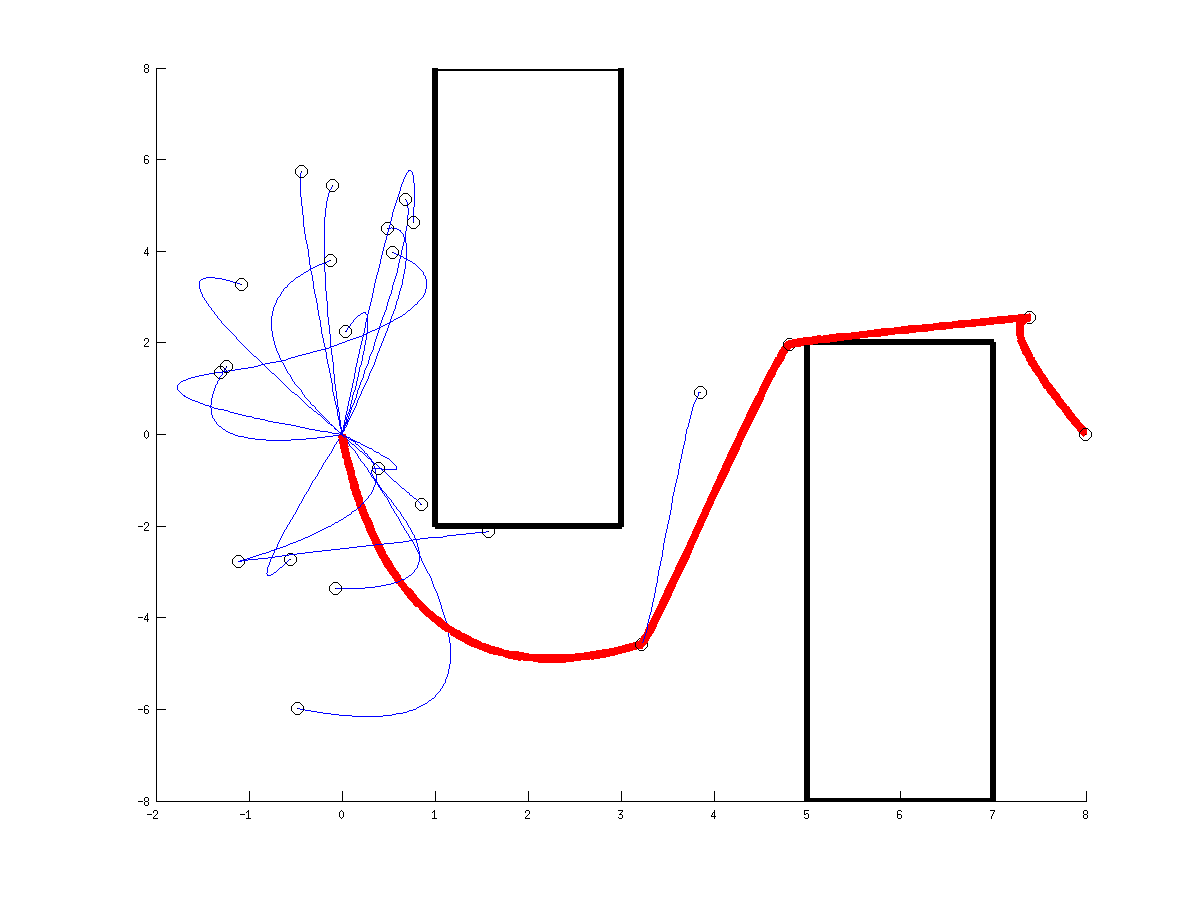
\includegraphics[width=1.6in]{diff_rrtstar5_1.png}}
    \subfigure[]{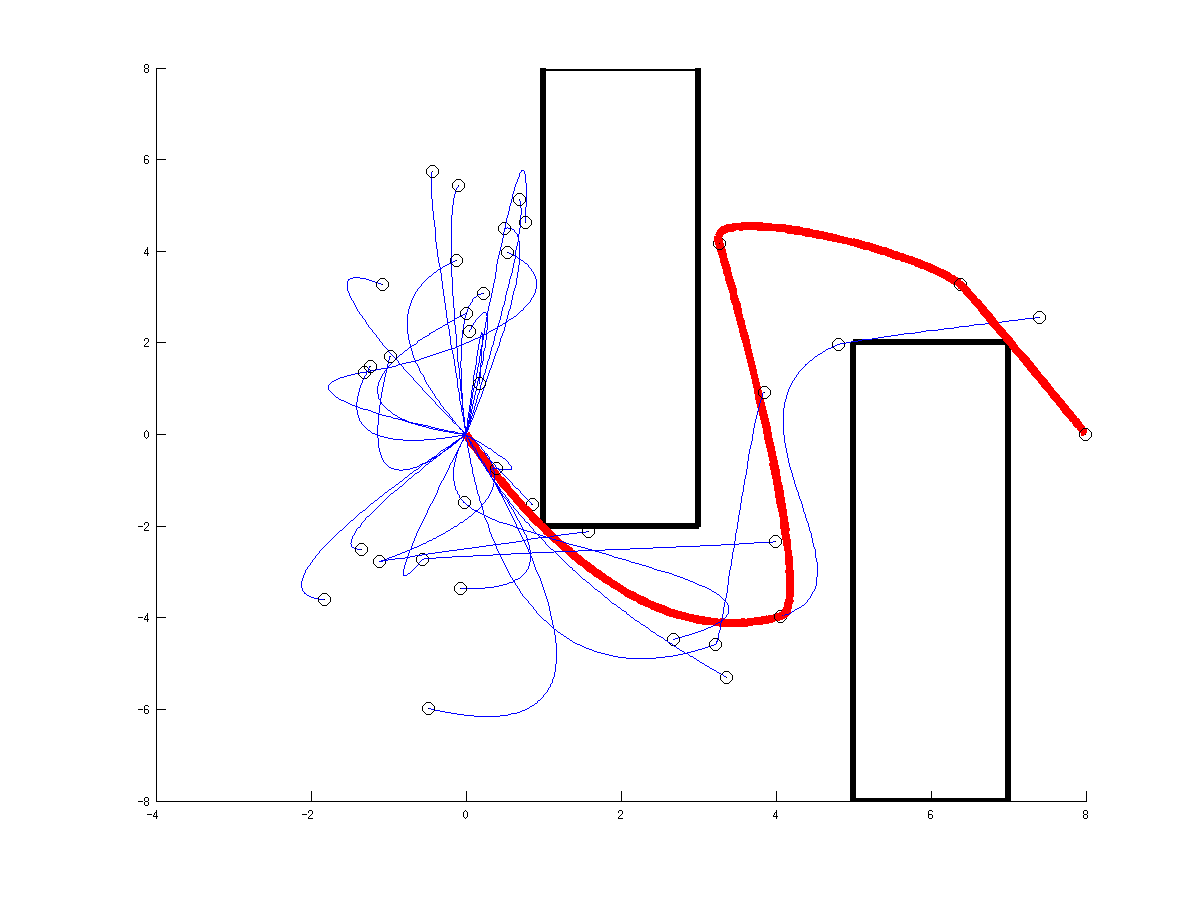
\includegraphics[width=1.6in]{diff_rrtstar5_3.png}}
    \subfigure[]{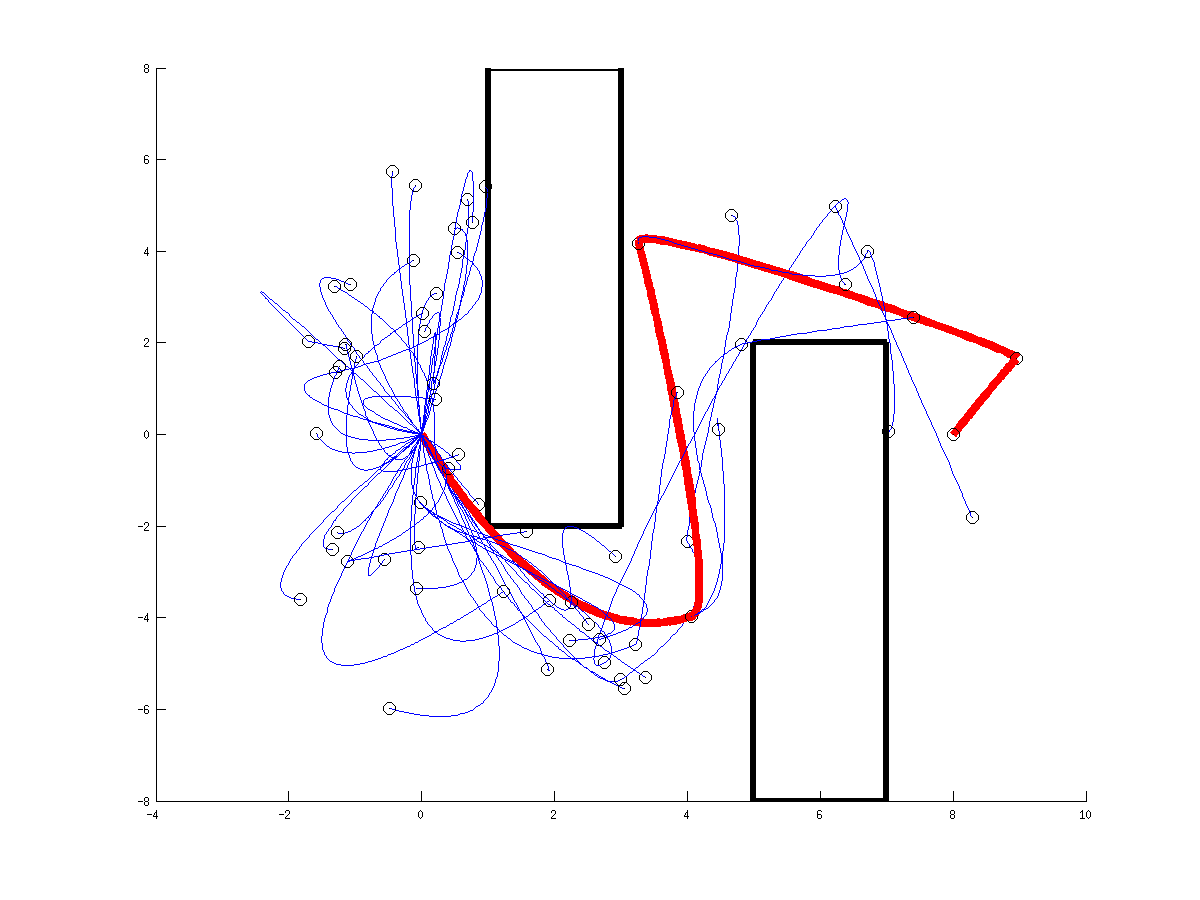
\includegraphics[width=1.6in]{diff_rrtstar5_5.png}}
    \subfigure[]{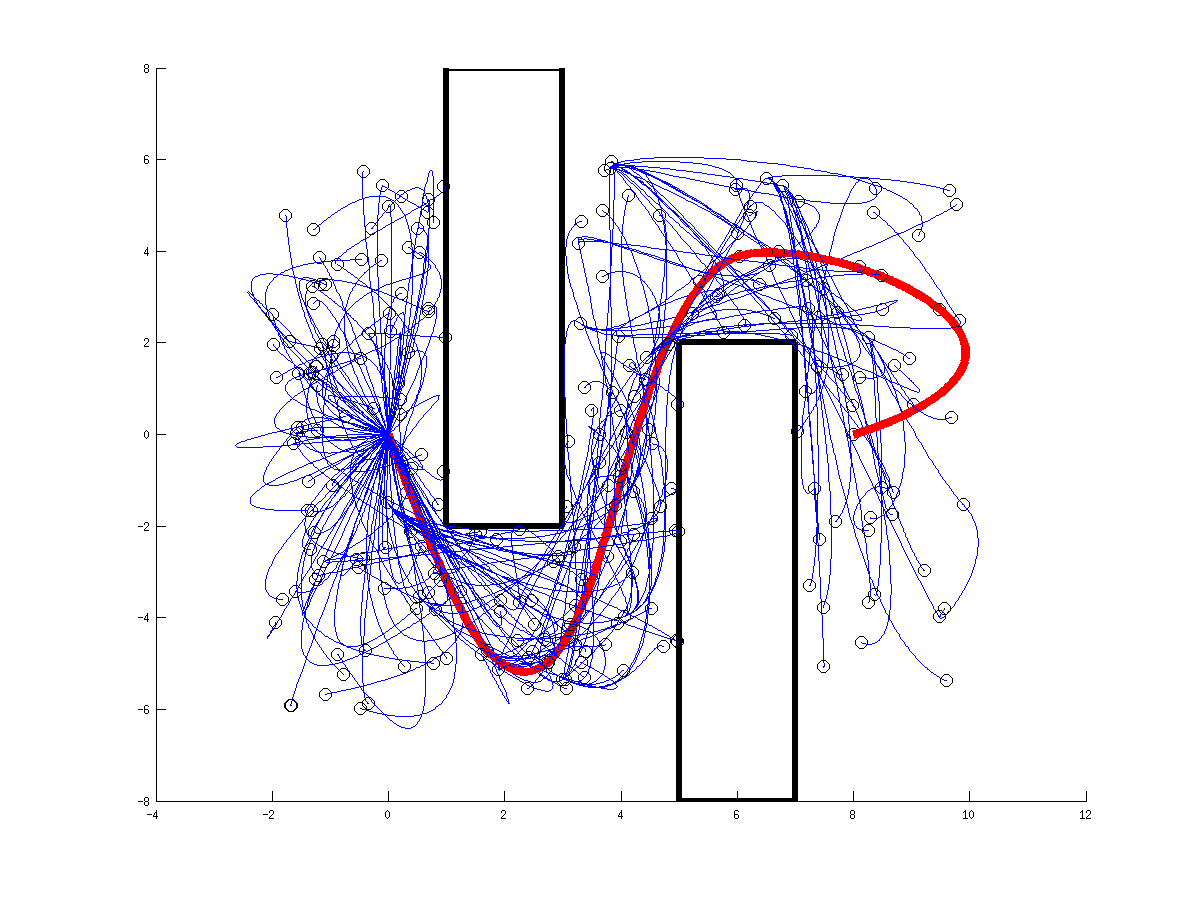
\includegraphics[width=1.6in]{diff_rrtstar5_9.png}}
  \end{center}
\end{center}
\caption{Example of using LQR-RRT$^*$ to find an optimal solution to
  the kinodynamic motion planning for the double integrator in the
  presence of obstacles. The four images show the tree at different
  points during growing. The blue lines show the tree. The red path
  denotes the current best path to the goal. The cost of the best path
  in each of the four frames is, respectively, 3515, 2495, 53, and
  14.}
\label{fig:linear_case_study}
\end{figure*}

We evaluated our approach to affine systems control using a
two-dimensional double integrator. Similar evaluations of RRT$^*$
performance for the double integrator have appeared
in~\cite{Karaman.Frazzoli:CDC10}
and~\cite{jur}. Figure~\ref{fig:linear_case_study} illustrates
the working of the algorithm for an example domain. Starting at
$(0,0)$ with zero velocity at time $t=0$, the system must reach the
goal at $(8,0)$ at time $t=10s$. The cost function
(Equation~\ref{eqn:affine_lqr_cost_nofinal}) has $Q=0$ and
$R=I$. After 600 iterations of the RRT$^*$ algorithm, there are 249
vertices in the tree and the current best-cost path has been improved
eight times. Initially, the algorithms finds a trajectory
(Figure~\ref{fig:linear_case_study}(a)) with cost $3515$. The
subsequent eight best-cost trajectories have costs $2495$, $2495$,
$215$, $53$, $47$, $27$, $22$, and $14$.

\begin{figure}
\begin{center}
  \begin{center}
    \subfigure[]{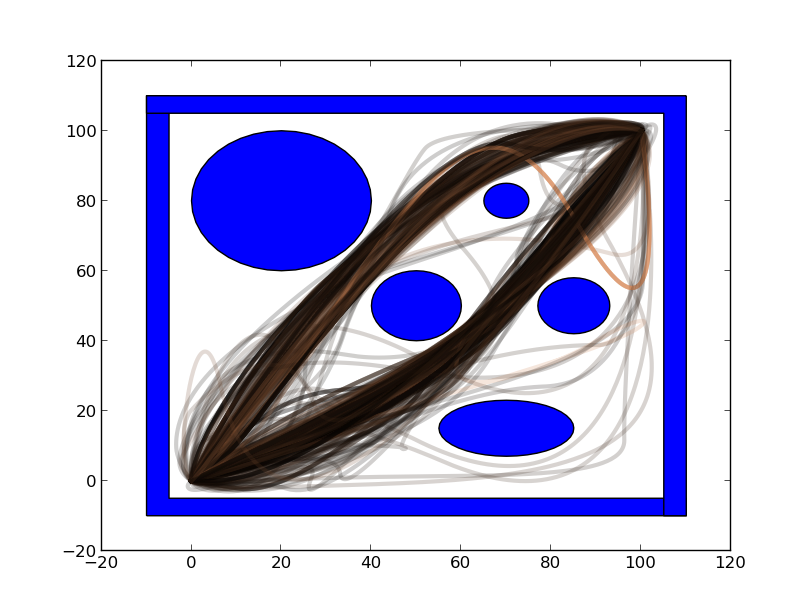
\includegraphics[width=2.4in]{rrt-2D-di_50-runs_sols.png}}
    \subfigure[]{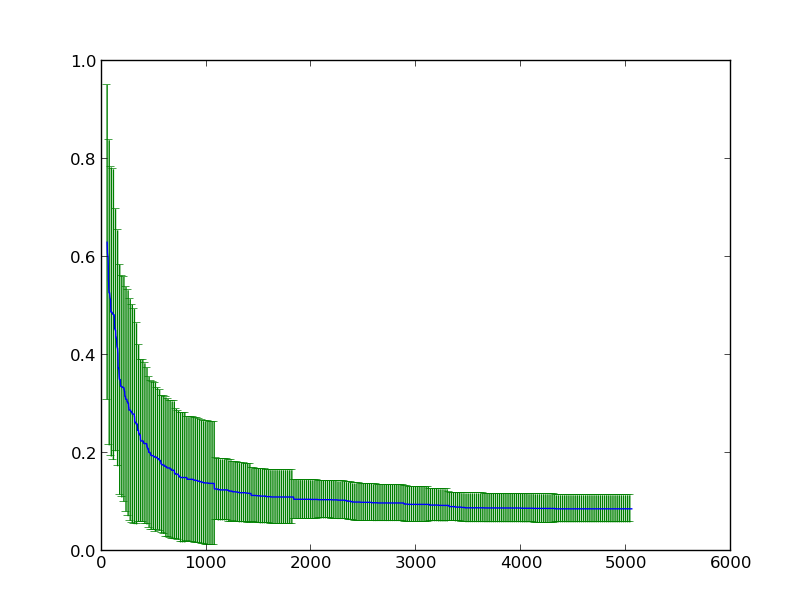
\includegraphics[width=2.4in]{rrt-2D-di_50-runs_convergence.png}}
  \end{center}
\end{center}
\caption{(a) Best-cost trajectories found during 50 separate runs of
  the algorithm. Darkness of the line is inversely proportional to
  trajectory cost. (b) Average and standard deviations of the costs of
  the best trajectories as a function of algorithm iteration number.}
\label{fig:linear_case_study2}
\end{figure}

We also evaluated average performance over multiple runs of the
algorithm
(Figure~\ref{fig:linear_case_study2}). Figure~\ref{fig:linear_case_study2}(a)
shows the set of best paths during 50 different runs of the algorithm
for the double integrator domain shown. Notice that the different runs
of the algorithm tend to identify two different homotopies that have
nearly equal costs. Figure~\ref{fig:linear_case_study2}(b) shows the
mean and standard deviations of the best-cost paths as a function of
algorithm iteration.



\section{Application to General Dynamical Systems}

Consider a discrete-time dynamical system in the form
\begin{equation}
x_{k+1}=f\left(x_{k},u_{k}\right)\label{eq:dynamics}
\end{equation}


with additive cost function
\begin{equation}
J\left(\mathbf{u},\mathbf{x}\right)=\sum_{k=0}^{T}g\left(x_{k},u_{k}\right)\label{eq:cost_functional}
\end{equation}


and starting point $x_{0}$. The state vector, $x$, is $n$-dimensional
and the control vector, $u$, is $m$-dimensional. We aim to find
a sequence $ $$\mathbf{u}=\left\{ u_{0},\cdots,u_{T}\right\} $ which
induces a trajectory $\mathbf{x}=\left\{ x_{1},\cdots,x_{T}\right\} $
satisfying the dynamics (\ref{eq:dynamics}) such that $ $$C$ is
minimized according to (\ref{eq:cost_functional}).

The real cost of moving from point $x'$ to $x''$ is
\begin{multline*}
C\left(x,x'\right)=\min_{\mathbf{u}}J\left(\mathbf{u},\mathbf{x}\right)\\
\mbox{subject to (\ensuremath{\ref{eq:dynamics}}), \ensuremath{x_{0}=x}, \ensuremath{x_{T}=x'}}
\end{multline*}


Note that the minimization happens over control sequences $\mathbf{u}$
of a fixed time lengths, according to

We approximate $C\left(x',x''\right)$ by taking a first-order approximation
of the dynamics and a second-order approximation of the cost and applying
LQR control. In general, the approximated dynamics and cost are of
the following form

\begin{align}
x_{k+1} & \approx Ax_{k}+Bu_{k}+c\label{eq:dynamics_approx}\\
J\left(\mathbf{u},\mathbf{x}\right) & \approx\sum_{k=0}^{T}x_{k}^{T}Qx_{k}+u_{k}^{T}Ru_{k}+2q^{T}x_{k}+2r^{T}u_{k}+d\label{eq:cost_approx}
\end{align}


$A$ and $Q$ are $n\times n$, $B$ is $m\times n$, $R$ is $n\times n$.
$c$ and $q$ are $n\times1$, $r$ is $m\times1$ and $d$ is a scalar.

\begin{align*}
A & =\left.\frac{\partial f}{\partial x}\right|_{x^{*},u^{*}}\\
B & =\left.\frac{\partial f}{\partial u}\right|_{x^{*},u^{*}}\\
c & =-Ax^{*}-Bu^{*}+f\left(x^{*},u^{*}\right)
\end{align*}


$x^{*}$, $u^{*}$ is the point about which the linearization is performed.
Typically $u^{*}$ is taken to be $\mathbf{0}$ and $x^{*}=x'$

Equations \ref{eq:dynamics_approx} and \ref{eq:cost_approx} are
the truncated Taylor expansions of $f$ and $g$. The dynamics $f$
must be once-differentiable and addition cost $g$ must be twice-differentiable.


\subsection{Reduction to the Previous Problem}

It is possible to transform the problem specified with \ref{eq:dynamics_approx}
and \ref{eq:cost_approx} into LQR form (where there is only an $A$,
$B$, $Q$, $R$ matrix) using the following:

\begin{align*}
\underbrace{\left[\begin{matrix}x_{k+1}\\
1
\end{matrix}\right]}_{\hat{x}_{k+1}} & =\underbrace{\left(\begin{matrix}A & c-R^{-1}r\\
0 & 1
\end{matrix}\right)}_{\hat{A}}\underbrace{\left[\begin{matrix}x_{k}\\
1
\end{matrix}\right]}_{\hat{x}_{k}}+\underbrace{\left(\begin{matrix}B\\
0
\end{matrix}\right)}_{\hat{B}}\hat{u}_{k}\\
C\left(\mathbf{u},\mathbf{x}\right) & =\sum_{k=0}^{T}\hat{x}_{k}^{T}\hat{Q}\hat{x}_{k}+\hat{u}_{k}^{T}R\hat{u}_{k}
\end{align*}


with $\hat{u}_{k}=u_{k}+R^{-1}r$ and $\hat{Q}=\left(\begin{matrix}Q & q\\
q^{T} & d
\end{matrix}\right)$ .

\begin{comment}
$\left(\begin{matrix}x\\
1
\end{matrix}\right)^{T}\left(\begin{matrix}Q & q\\
q^{T} & \eta_{1}
\end{matrix}\right)\left(\begin{matrix}x\\
1
\end{matrix}\right)=\left(\begin{matrix}x\\
1
\end{matrix}\right)^{T}\left(\begin{matrix}Qx+q\\
q^{T}x+\eta_{1}
\end{matrix}\right)=x^{T}Qx+x^{T}q+q^{T}x+d$
\end{comment}


The $\hat{A}$, $\hat{B}$, $\hat{Q}$, and $R$ matrices specify
a linear dynamical system with quadratic costs to which an optimal
solution can be found with LQR.


\subsection{Nuances and Subtleties}


\subsubsection{Non-exact steering}

rewiring and propagating dynamics


\subsubsection{Uncontrollable Dynamics}

The linearized system may be uncontrollable -- the $A$ and $B$ matrices
are such that it's not possible to control all the modes of the system.
This is the case, for example, for a cart with two inverted pendulums
of the same length linearized about the upward-pointing fixed point.
The control input to the system affects both linearized pendulums
in the same way, so it's not possible to independently stabilize them.
For the infinite-horizon LQR control problem, there is no solution.
For the finite-horizon problem, there is a solution, though it might
not be possible to go to any arbitrary location. If the system linearized
at $x'$ cannot reach $x''$, then $C\left(x',x''\right)$ needs to
be defined in another way.

is Therefore using the LQR cost metric cannot approximate the cost

\begin{comment}
Typical RTT{*} the cost metric is an underestimate of the true cost,
since the metric does not take into consideration obstacles. The true
cost, for example, might be infinite if there is no feasible path,
but the Euclidian metric will always be finite.

If the system is uncontrollable as is linearized by a single point,
then the LQR cost will be infinite while the true cost is not.
\end{comment}



\subsubsection{Indefinite Cost}

\begin{comment}
What if $\hat{Q}$ is indefinite?

Options:

1. Use sequential QP techniques like shifting eigenvalues to make
$\hat{Q}$ definite.

http://www.cs.berkeley.edu/\textasciitilde{}pabbeel/cs287-fa11/slides/NonlinearOptimizationForOptimalControl.pdf
(Page 11 bottom slide)

2. LQR with indefnite weighting matrices

Chapter 9 of:

http://epubs.siam.org.libproxy.mit.edu/doi/book/10.1137/1.9781611970760

(same book)

http://books.google.com/books?id=bD\_83idGZ2cC\&lpg=PA211\&ots=q3U7u4rmNc\&dq=indefinite\%20LQR\&pg=PA211\#v=onepage\&q\&f=false

http://www.tandfonline.com/doi/abs/10.1080/00207178408933184\#preview
\end{comment}



\subsubsection{Actuation Constraints}

The LQR framework does not permit actuation constraints.

\begin{comment}
Say the LQR solution returns a control action $u\not\in\mathcal{U}$
(the set of permitted actions). Simply choosing a $u'=\alpha u$ such
that $u'\in\mathcal{U}$ while minimizing $\alpha^{2}$ (so that $u'$
is close to $u$) intuitively will not explore the space as desired
-- the state won't move along the same direction in general.

To clarify:

if the state of the system is $x_{k}$, then the next state is $x_{k+1}=Ax_{k}+Bu$,
which presumably moves the system toward $x_{rand}$. The state $x_{k+1}'=Ax_{k}+Bu'$
does not, in general, move the system directly toward $x_{rand}$.
\end{comment}



\subsubsection{Asymmetric Cost}

\begin{comment}
http://math.stackexchange.com/a/23397/2256
\end{comment}



\subsection{Non-linear Domain}

spaceship orientation


\subsection{Results}

Quick mention of performance (or not). Picture of tree, cost over
iteration


\section{Discussion and Conclusion and Future Work}

Code available. Spatial Data structure future


\section{Acknowledgments}


\section{References}
\bibliographystyle{IEEEtran}
\bibliography{references}
\end{document}
